\documentclass[hidelinks, 11pt]{article}

\title{AMATH 271: Final Project}
\author{Omer Sipra, Kamalesh Reddy}

\usepackage[letterpaper,margin=1in]{geometry}
\usepackage{graphicx}
\usepackage{hyperref}
\usepackage{amsmath}
\usepackage{amssymb}
\usepackage{bm}
\usepackage{listings}
\usepackage{color}
\usepackage{tikz}
\usetikzlibrary{decorations.pathreplacing,shapes.misc}
\usepackage{hologo} % or use package holog?

\usepackage{empheq}
\usepackage{color}
%\usepackage{parallel,enumitem}
%\usepackage{textgreek}

\usepackage[T1]{fontenc}
\usepackage{textcomp}
\lstset{upquote=true}

\lstset{
  literate={∂}{{$\partial$}}1
           {ℒ}{{$\mathcal{L}$}}1
           {φ}{{$\phi$}}1
}

\UseRawInputEncoding
\usetikzlibrary{decorations.pathmorphing,patterns}

\definecolor{myblue}{rgb}{.92549, .98824, 0.95686}
\newlength\mytemplen
\newsavebox\mytempbox

\makeatletter
\newcommand\mybluebox{%
\@ifnextchar[%]
{\@mybluebox}%
{\@mybluebox[0pt]}}

\def\@mybluebox[#1]{%
\@ifnextchar[%]
{\@@mybluebox[#1]}%
{\@@mybluebox[#1][0pt]}}

\def\@@mybluebox[#1][#2]#3{
\sbox\mytempbox{#3}%
\mytemplen\ht\mytempbox
\advance\mytemplen #1\relax
\ht\mytempbox\mytemplen
\mytemplen\dp\mytempbox
\advance\mytemplen #2\relax
\dp\mytempbox\mytemplen
\colorbox{myblue}{\hspace{1em}\usebox{\mytempbox}\hspace{1em}}}

\makeatother

\definecolor{dkgreen}{rgb}{0,0.6,0}
\definecolor{gray}{rgb}{0.5,0.5,0.5}
\definecolor{mauve}{rgb}{0.58,0,0.82}

\lstset{frame=tb,
language=Python,
aboveskip=3mm,
belowskip=3mm,
showstringspaces=false,
columns=flexible,
basicstyle={\small\ttfamily},
numbers=none,
numberstyle=\tiny\color{gray},
keywordstyle=\color{blue},
commentstyle=\color{dkgreen},
stringstyle=\color{mauve},
breaklines=true,
breakatwhitespace=true,
tabsize=3
}

\newcommand{\Lagr}{\mathcal{L}}

\def\changemargin#1#2{\list{}{\rightmargin#2\leftmargin#1}\item[]}
\let\endchangemargin=\endlist 

\newcommand\blfootnote[1]{%
  \begingroup
  \renewcommand\thefootnote{}\footnote{#1}%
  \addtocounter{footnote}{-1}%
  \endgroup
}

\begin{document}

\maketitle

\begin{center}
  \noindent\rule{16cm}{0.4pt}
  \section*{Abstract} %\cite{Taylor2005}}
  \noindent\rule{16cm}{0.4pt}
\end{center}

\begin{changemargin}{1cm}{1cm}
\textit{The following project falls in the mathematical domain of Calculus of Variation. It exhibits a computer program that is designed to provide a path of least "insert independent variable here" for any problem in Theoretical Mechanics. The computer program uses principles from Lagrangian Mechanics to achieve this. The problem’s lagrangian (specifically, it's arguments) is the input to the program and, using the Euler-Lagrange equation, the programs provide the user with a plot of the minimized quantity vs the independent variable that they defined.}
\end{changemargin}

\begin{center}
  \noindent\rule{16cm}{0.4pt}
  \section*{Introduction} %\cite{Taylor2005}}
  \noindent\rule{16cm}{0.4pt}
\end{center}

The problem that inspired this Project is one of the oldest problems in Calculus of Variations. The problem was a challenge by the mathematician Johann Bernoulli. He described the problem as:
“Given two points A and B in a vertical plane, what is the curve traced out by a particle under the influence of gravity (constant), which starts at A and reaches B in the shortest time.”

In other words: 'A' is any arbitrary point ($x_{0}$, $y_{0}$) in 2 dimensional space and B is defined as ($x_{1}$, $y_{1}$) where $y_{1} \leq y_{0}$ and $x_{0} \neq x_{1}$. This results in B being a translation of A which is under (but not directly under A). The system includes a particle which is supposed to “fall” from A to B because of a constant gravitational force. The objective of the problem is to find the path that would require the least time for the particle to get to B. 

The problem was attempted and successfully solved by several mathematicians. Isaac Newton famously solved the problem overnight. The solution of this problem was named the “Brachistochrone”.  Johann Bernoulli’s solution being the first, identified this brachistochrone to be the common cycloid. 

% \begin{figure}
%     \centering
%     \includegraphics[width=0.5\columnwidth]{Cycloid.jpg}
%     \caption{Cycloid \cite{Carnier2017}}
%     \label{Cycloid}
% \end{figure}

A cycloid is the path traced out by a point on the circumference of a circle as it rolls on a horizontal surface without slipping. 

Different solutions to this problem were developed until as early as the 2010's. One of these solutions is what inspired this project. It was developed by Mark Levi \cite{Levi2014} in 2014. His solution shows this symmetry in the path of least time called the “tautochrone” property of a brachistochrone, which means that the path a particle would take to fall from any point on the cycloid to B would all be the same! This made us realize that for any mechanical problem there exists 1 solution that describes the path of a least quantity which can be scaled to any magnitude of the problem’s dimensions. 

Another solution to the brachistochrone problem is provided in the textbook \cite{Taylor2005}. It involves finding the Lagrangian of the problem and using the Euler-Lagrange equation to find a DE that can be plotted. The resulting plot, as expected, reveals a brachistochrone.

If this method works for the brachistochrone problem, then it should work for any arbitrary problem in mechanics where a path can be traced. 
We hence decided to create a program to find the path of least time/distance of any problem that involves a Lagrangian. To achieve this we used the solutions mentioned above to design a program written in Python that can take a Lagrangian input (which corresponds to a mechanics problem of course) and then said code will show you the path of least distance/time. 
To demonstrate this project we tested the program for a couple of problems including problems from Mini-Project 2, AMATH 271 and problems from chapter 6 of Taylor.
The first two problems of the project are borrowed from Taylor. The first problem is the simplest on the project and helped us understand how to setup the mechanics of the code. It requires us to find the shortest possible path between two points using the Euler-Lagrange method. We know that the answer to this is a straaight line. The problem verifies this by using the arc length measurement and minimizing the distance through that, On the other hand, the second problem is the brachistochrone problem itself, but following the same method as problem 1. We are supposed to find the path of least time to get from A to B (A and B being the points defined above). This problem also involves inverting out independent and dependent variable which is something the code would have to account for to work in all problems. 

The last 2 problems of the project were borrowed from Mini Project 2. These problems are a lot more complex than the first two and use conventional method of finding a Lagrangian to then minimize a quantity. Since we already knew the solutions to these, they served as a good way to find potential shortcomings of our method and also verified anything we did right, 

Following are out findings and the code:

\newpage

%\section{hello}
\begin{center}
  \section*{1}
  \noindent\rule{16cm}{0.4pt}
  \section*{Taylor Example 6.1: Shortest Path Between 2 Points (warm-up)} %\cite{Taylor2005}}
  \noindent\rule{16cm}{0.4pt}
\end{center}

\subsection*{1.1 Equations of problems}

\begin{center}
  \begin{tikzpicture}
    \node at (0, -0.35) {$(x_0, y_0)$};
    \node at (5, -0.6) {$(x_1, y_1)$};
    \draw [black, dotted]  (0,0) -- (5,-1);
    \draw [black] plot [smooth, tension=2] coordinates {(0,0) (1,1) (2,-1) (5,-1)};
  \end{tikzpicture}
\end{center}

%\textbf{$\mathcal{L}$}\textit{\textbf{agrangian}}

\noindent Now, consider a small section of the curve, ds (an arbitrarily small ds is a line): 

\begin{center}
  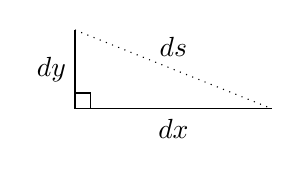
\begin{tikzpicture}
    \draw [dotted] (0, 1) -- (5/2, 0);
    \draw (0, 0) -- (0, 1);
    \draw (0, 0) -- (5/2, 0);
    \node at (-0.3, 1/2) {$dy$};
    \node at (5/4, -0.25) {$dx$};
    \node at (5/4, 1/2 + 0.29) {$ds$};
    \draw (0.2, 0) -- (0.2, 0.2);
    \draw (0, 0.2) -- (0.2, 0.2);
  \end{tikzpicture}
\end{center}

We can hence write ds in terms of small steps in the x and y direction using the Pythagorean theorem:\newline 

  $ds^2 = dx^2 + dy^2 \implies ds = \sqrt{dx^2 + dy^2} \implies ds = \sqrt{1 + \left(\cfrac{dy}{dx} \right)^2}\,dx \implies ds = \sqrt{1 + y'(x)^2}\,dx $

Integrating on both sides from $(x_0, y_0)$ to $(x_1, y_1)$:
\begin{center}
  $\displaystyle\int_{(x_0, y_0)}^{(x_1, y_1)} \,ds = \int_{x_0}^{x_1} \sqrt{1 + \dot{y}^2}\,dx$.
\end{center}
  %\begin{center}
  %$\Lagr(x,y,y') = f(x,y,y') = \sqrt{1+y'^2}$
  %\end{center}

\subsection*{1.2 Analysis}
Our goal is to minimize the integral, $\displaystyle\int_{(x_0, y_0)}^{(x_1, y_1)} \,ds$.
To minimize this, observe that, equivalently, we can take the integrand, $\sqrt{1 + \dot{y}^2}$, to be our Lagrangian (the proof of which is omitted)\footnote[1]{Look into "Calculus of variations", Euler-Lagrange equation", and "Principle of stationary action".}. This is the essence of Lagrangian mechanics, it says nature is an optimization problem and depicts ``nature is lazy" in equations. We have, 

\begin{empheq}[box={\mybluebox[5pt][5pt]}]{equation*}
  \Lagr(\dot{y}, y, x) = \sqrt{1 + \dot{y}^2}
\end{empheq}
\\

\subsection*{1.3 Solutions - \emph{SPBTP.py}}
Now, on to solving this problem! Now that we have the Lagrangian, we can feed it to our Python program while making necessary changes (passing parameters (here, constants), variables `names', and the Lagrangian itself as parameters).

\noindent The mechanism of this program will be explained in detail for this warm-up problem:
\newline

\begin{changemargin}{2cm}{2cm}
  \begin{enumerate}
    \item We import the required libraries; in this program, we will only need \verb|sympy| to output the derivative. However, we will not use it to solve the derivative, since most derivatives cannot be solved numerically, which is how sympy solves them. We will use a second program to solve the derivative numerically.
    \item Declare the function, \verb|givemeDE|. The function does not explicitly take the lagrangian as an argument (for reasons that I will state later); BUT, the lagrangian is defined locally in the very next step, this makes it easier for the user to define the lagrangian, which will be required either way.
    \item This problem's lagrangian does not require us to define any parameter (clearly).
    \item The user must define the lagrangian, \verb|L|, manually.
    \newline
    \textit{Note: Make sure the Lagrangian is a function of \textbf{three} variables.}
    \item We then assign each variable; the dependent variable's derivative, the dependent variable, and the independent variable; with strings. This displays the differential equation with appropriate strings in place of \verb|dvarp|, \verb|dvar|, and \verb|ivar| (the general variables our program uses).
    \item The next step is where Python solves for each term of the lagrangian and \verb|prints| it to the console. 
    \item Then, it plugs the two terms into the Euler-Lagrange equation (defined implicitly) and isolates all terms.
    \item Finally, it prints the \verb|DE|. The final differential equation will be of the form $f(\dot{q}, q, t) = 0$.
    \item Keep the format of the function \verb|givemeDE| in mind.
  \end{enumerate}
\end{changemargin}
Crux: the program take the lagrangian as ``input" and gives us the DE: $f(\ddot{q}, \dot{q}, q, t) = 0$. This DE will now be solved, again, using Python. Running the code below (\verb|derog.py|) as is, we get:

\begin{lstlisting}[language = html]
∂ℒ/∂y        = 0


∂ℒ/∂y'       = Derivative(y(x), x)/sqrt(Derivative(y(x), x)**2 + 1)


d/dx(∂ℒ/∂y')  = Derivative(y(x), (x, 2))/sqrt(Derivative(y(x), x)**2 + 1) - Derivative(y(x), x)**2*Derivative(y(x), (x, 2))/(Derivative(y(x), x)**2 + 1)**(3/2)
Required DE: y''/(y'**2 + 1)**(3/2) = 0
\end{lstlisting}   
$\verb|y''/(y'**2 + 1)**(3/2) = 0| \implies \ddot{y} = 0:$ (This is, as expected, a straight line!)
\begin{empheq}[box={\mybluebox[0pt][0pt]}]{equation*}
  y(x) = C_1 + C_2x
\end{empheq}
\newpage

  


\begin{lstlisting}[frame = none]
  Python Code:
\end{lstlisting}

\begin{lstlisting}[frame = left]
  # LIBRARIES
  import sympy as sp

  # FUNCTION
  def givemeDE(*args):
    
    #PARAMETERS

    #LAGRANGIAN
    def L(dvar, dvarp, ivar):
        return sp.sqrt(1 + dvarp**2)
    
    if len(args) == 3:
        # AESTHETICS
        def convertEq(x):
            x = x.replace("Eq(", "")
            x = x.replace(", 0)", "")
            x = x + " = 0"
            return x
        # AESTHETICS
        def convertDE(de):
            de_str = str(de)
            de_str = de_str.replace("Derivative(" + args[-2] + "(" + args[-1] + "), (" + args[-1] + ", 2))", args[-3] + "'" + "'")
            de_str = de_str.replace("Derivative(" + args[-2] + "(" + args[-1] + "), " + args[-1] + ")", args[-3] + "'")
            de_str = de_str.replace(args[-2] + "(" + args[-1] + ")", args[-3])
            return de_str

        # DEFINES ASSIGNED SYMBOLS
        ivar = sp.Symbol(args[-1])
        dvar = sp.Function(args[-2])(ivar)
        dvarp = sp.Derivative(dvar, ivar)

        # PRINTS EACH TERM OF THE LAGRANGIAN
        print("∂ℒ/∂" + args[-3] + "        =", sp.diff(L(dvar, dvarp, ivar), dvar))
        print('\n')         
        print("∂ℒ/∂" + args[-3] + "'" + "       =", sp.diff(L(dvar, dvarp, ivar), dvarp))
        print('\n')         
        print("d/d" + args[-1] + "(∂ℒ/∂" + args[-3] + "')" + "  =", sp.diff(sp.diff(L(dvar, dvarp, ivar), dvarp), ivar))

        # FINDS DE USING TERMS ABOVE
        de = sp.simplify(sp.Eq(sp.diff(L(dvar, dvarp, ivar), dvar) - sp.diff(sp.diff(L(dvar, dvarp, ivar), dvarp), ivar), 0))

        # PRINTS OUT DE
        print("Required DE:", convertDE(convertEq(str(de))))

# EXECUTE PROGRAM!
givemeDE("y", "y", "x")
\end{lstlisting}

%\section{hello}
\begin{center}
  \section*{2}
  \noindent\rule{16cm}{0.4pt}
  \section*{Taylor Example 6.2: Brachistochrone} 
  \begin{changemargin}{3.7cm}{3.7cm}
    ``Given two points A and B in a vertical plane, what is the curve traced out by a point acted on only by gravity, which starts at A and reaches B in the shortest time.'' - \emph{Johann Bernoulli}
  \end{changemargin}
  \noindent\rule{16cm}{0.4pt}
\end{center}

\subsection*{2.1 Equations of problems}

\begin{center}
  \begin{tikzpicture}
  \coordinate (O) at (0,0);
  \coordinate (A) at (0,-2);
  \def\r{1} % radius
  \def\c{1.4} % center
  \coordinate (C) at (\c, \r);

  \node at (0, 0.4) {$(x_0, y_0)$};
  \node at (6.28, 0.4) {$(x_1, y_1)$};
  \draw[-latex] (O) -- (A) node[anchor=north] {$y$};
  \draw[-latex] (O) -- (2.6*pi,0) node[anchor=west] {$x$};
  \draw[black,domain=0*pi:2*pi,samples=100, line width=0.1] 
       plot ({\x - sin(\x r)},{cos(\x r)- 1});

  % coordinate x 
  \def\x{0.4} % coordinate x
  \def\y{0.83} % coordinate y
  \def\xa{0.3} % coordinate x for arc left
  \def\ya{1.2} % coordinate y for arc left
  
  \end{tikzpicture}
\end{center}
%\textbf{$\mathcal{L}$}\textit{\textbf{agrangian}}

Now that we know how to minimize a certain quantity numerically using the Euler-Lagrange equations, we will follow the same method in solving this problem. We have:

\begin{center}
$v = \sqrt{2gy} \implies \cfrac{ds}{dt} = \sqrt{2gy}$
\end{center}

Since we want to minimize time, we isolate $`dt'$:

\begin{center}
  $dt = \cfrac{ds}{\sqrt{2gy}}$
\end{center}

From Section 1.1, we know that $ds = \sqrt{1 + x'(y)^2}$. On substitution:

\begin{center}
  $dt = \cfrac{\sqrt{1 + x'(y)^2}\,dx}{\sqrt{2gy}}$
\end{center}

Integrating on both sides from initial point to final point:

\begin{center}
  $\displaystyle\int_{t_0}^{t_1} \,dt = \int_{x_0}^{x_1} \cfrac{\sqrt{1 + x'(y)^2}}{\sqrt{2gy}}\,dx$
  $\implies \displaystyle\int_{t_0}^{t_1} \,dt = \cfrac{1}{\sqrt{2g}}\int_{x_0}^{x_1} \sqrt{\cfrac{1 + x'(y)^2}{y}}\,dx$.
\end{center}

\newpage

\subsection*{2.2 Analysis}

According to our problem statement, we want to minimize the time, $\displaystyle\int_{t_0}^{t_1} \,dt$. We procced in the same way (Section 1.2), by choosing $\sqrt{\cfrac{1 + x'(y)^2}{y}}$ to be our lagrangian:

\begin{empheq}[box={\mybluebox[3pt][3pt]}]{equation*}
  \Lagr(\dot{x}, x, y) = \sqrt{\cfrac{1 + x'(y)^2}{y}}
\end{empheq}

\subsection*{2.3 Solutions - \emph{Brach.py}}

The entire program will not be explained since most of it remains the same; the only parts that change are: the definition of the lagrangian and the final DE that we will plot this time.

\noindent The Lagrangian is defined as follows:
\begin{lstlisting}
  def L(dvar, dvarp, ivar):
      return sp.sqrt((dvarp**2 + 1)/ivar)
\end{lstlisting}

\noindent Also note the change in variables, the independent variable here is $y$ and the dependent variable is $x$, so we change the arguments of the function as follows:

\begin{lstlisting}
givemeDE("x", "x", "y")
\end{lstlisting}

\noindent We must also comment out the line that prints the DE's solution. This is because sympy solves DE's analytically to output a cartesian equation, however, in the case of a brachistochrone there is no such equation (or it is rather complicated); we instead verify by solving it numerically and plotting the solution using the following code from \verb|DEnumerical.py|:

\begin{lstlisting}[frame = left]
import numpy as np
from scipy.integrate import odeint
import matplotlib.pyplot as plt

def brach(a):
    def diffeqs(w, y, p):
        [x] = w # d matrix
        [] = p # parameters
        der = [np.sqrt(y/(2*a - y))] #Spoiler Alert!
        return der

    # y values
    y = np.linspace(0.001, 2.1, 100000)

    # containing parameters and initial conditions
    p = []
    w0 = [0]

    wsol = odeint(diffeqs, w0, y, args = (p, ))
    plt.plot(wsol[:, 0], -1*y)
brach(1)
plt.show()
\end{lstlisting}

\noindent Brief explanation of the code above:
\begin{enumerate}
\item Again, we import the required libraries; in this program, we will need \verb|numpy| and \verb|scipy| to solve the DE numerically, and then we plot it using \verb|matplotlib.pyplot|.
\item \verb|brach(a)| is a function that takes `a', the parameter, as an argument.
\item \verb|diffeqs(w, y, p)| then solves the system of differential equations as per it's definition inside \verb|diffeqs| and returns the derivative of the matrix.
\item \verb|odeint| then uses \verb|diffeqs|; the initial conditions, \verb|w0|; the y (independent variable) values \verb|y|; and the parameters, here, `\verb|a|' to solve the system and store them in \verb|wsol|
\item Then, we simply plot $y vs. x$ or, here, \verb|(wsol[:, 0], -1*y)| after adjusting `direction' of y.
\end{enumerate}

\noindent Now that we have the code out of the way; let's find the DE numerically, we run the program to get:

\begin{lstlisting}[language = html]
  ∂ℒ/∂x        = 0


  ∂ℒ/∂x'       = sqrt((x'**2 + 1)/y)*x'/(x'**2 + 1)
  
  
  d/dy(∂ℒ/∂x')  = y*sqrt((x'**2 + 1)/y)*(x'*x''/y 
                 - (x'**2 + 1)/(2*y**2))*x'/(x'**2 + 1)**2 
                 + sqrt((x'**2 + 1)/y)*x''/(x'**2 + 1) 
                 - 2*sqrt((x'**2 + 1)/y)*x'**2*x''/(x'**2 + 1)**2
  
  
  Required DE      : (-2*y*x'' + x'**3 + x')/(2*y**2*sqrt((x'**2 + 1)/y)*(x'**2 + 1)) = 0
  \end{lstlisting}  

\noindent Now, observe that \verb|d/dy|$(\partial \Lagr/\partial x')$ looks rather complicated. Instead, as suggested in Taylor we can say that since $\partial \Lagr/\partial x = 0$, \verb|d/dy|$(\partial \Lagr/\partial x') = 0 \implies \partial \Lagr/\partial x' = C$, where $C$ is the constant of integration;

\begin{center}
$\implies$ \verb|sqrt((x'**2 + 1)/y)*x'/(x'**2 + 1)|  $= \sqrt{\cfrac{x'^2 + 1}{y}}\cdot\cfrac{x'}{x'^2+1} = \cfrac{x'}{\sqrt{y(x'^2+1)}} = C$
\end{center}

\noindent Setting $C = \sqrt{\cfrac{1}{2r}}$ (as we will see later, r is the radius of the cycloid's circle):

\begin{center}
$\cfrac{x'^2}{y(x'^2+1)} = C^2 \implies \cfrac{x'^2}{y(x'^2+1)} = \cfrac{1}{2r} \implies 2rx'^2 = y(x'^2+1) \implies x'^2(2r - y) = y$
\end{center}

\begin{empheq}[box={\mybluebox[5pt][10pt]}]{equation*}
  x' = \sqrt{\cfrac{y}{2r - y}}
\end{empheq}

\newpage

\noindent We solve the following ``system'' using \verb|DEnumerical.py|:                        

\begin{center}
$\left[x\right] = \left[\sqrt{\cfrac{y}{2r - y}}\,\,\right]$  
\end{center}

\noindent That is:

\begin{center}
\noindent \verb|      [x] = w|\newline
\verb|      [a] = p|\newline
\verb|      der = [np.sqrt(y/((2*a) - y))]|
\end{center}

\noindent For $a = 1$:
\begin{center}
  \makebox[0pt]{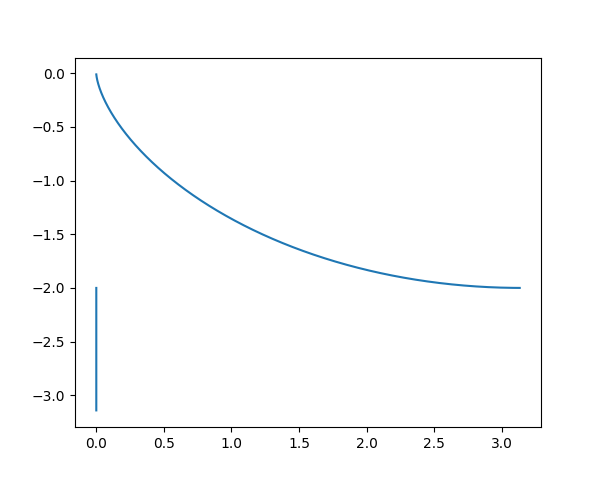
\includegraphics[scale=0.8]{brach(1).png}}

\begin{changemargin}{4.5cm}{4.5cm}  
  Figure 2.1: Cycloid with a circle of radius 1.
\end{changemargin}
\end{center}
\newpage

\begin{center}
  \section*{3}
  \noindent\rule{16cm}{0.4pt}
  \section*{Mini-Project 2: Question 1} %\cite{Taylor2005}}
  \noindent\rule{16cm}{0.4pt}
\end{center}

\subsection*{3.1 Equations of problems}

\begin{center}
  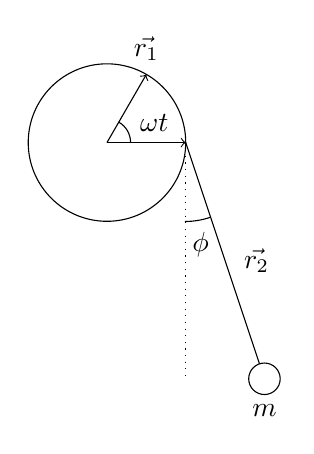
\begin{tikzpicture}
    \draw (0, 0) circle (1cm);
    \draw (1, 0) -- (2, -3);
    \draw [dotted] (1, 0) -- (1, -3);
    \draw (1.316, -0.948) arc (-71:-90:1);
    \node at (1.19, -1.3) {$\phi$};
    \node at (1.9, -1.5) {$\vec{r_2}$};
    \draw [fill=white] (2, -3) circle (0.2cm);
    \node at (2, -3.4) {$m$};
    \draw [->] (0, 0) -- (1, 0);
    \draw [->] (0, 0) -- (0.5, 1.73/2);
    \draw (0.3, 0) arc (0:60:0.3);
    \node at (0.5, 1.19) {$\vec{r_1}$};
    \node at (0.6, 0.25) {$\omega t$};
  
  \end{tikzpicture}
\end{center}
%\textbf{$\mathcal{L}$}\textit{\textbf{agrangian}}



\subsection*{3.2 Analysis}

From Mini-project 1, question 1; we have the following lagrangian for the above system:

$\Lagr = \Lagr(\phi', \phi, t) = \cfrac{m}{2}\, (R^2 \omega^2 + L^2 \dot{\phi}^2 + 2 R \omega L \dot{\phi}\sin(\phi - \omega t)) - mg(R \sin(\omega t) - L \cos(\phi))$ 

\subsection*{3.3 Solutions - \emph{.py}}

Plugging this Lagrangian into \verb|MP2q1.py|, the program retruns the DE, we get (for $\omega = 0$ and $0.2$):

\begin{lstlisting}[language = html]
  ∂ℒ/∂φ        = -1.0*sin(φ)  # w = 0


  ∂ℒ/∂φ'       = 1.0*φ'
  
  
  d/dt(∂ℒ/∂φ')  = 1.0*φ''
  
  Required DE      : 1.0*sin(φ) + 1.0*φ'' = 0
\end{lstlisting} 

\begin{lstlisting}[language = html]
  ∂ℒ/∂φ        = -1.0*sin(φ) + 0.04*cos(0.2*t - φ)*φ'  # w = 0.2


  ∂ℒ/∂φ'       = -0.04*sin(0.2*t - φ) + 1.0*φ'
  
  
  d/dt(∂ℒ/∂φ')  = -0.04*(0.2 - φ')*cos(0.2*t - φ) + 1.0*φ''
  
  Required DE      : 1.0*sin(φ) - 0.008*cos(0.2*t - φ) + 1.0*φ'' = 0
\end{lstlisting} 

\noindent $\omega = 0$:\\
\verb|1.0*sin(phi) + 1.0*phi'' = 0| \\
$\implies \phi'' = -\sin{\phi}$
\\
\noindent $\omega = 0.2$:\\
\verb|1.0*sin(phi) - 0.008*cos(0.2*t - phi) + 1.0*phi'' = 0| \\
$\implies \phi'' = -\sin{\phi} + 0.008\cos{(0.2t - \phi)}$

We hence get the following plots: (just as in Question 1!)

\begin{center}
  \makebox[0pt]{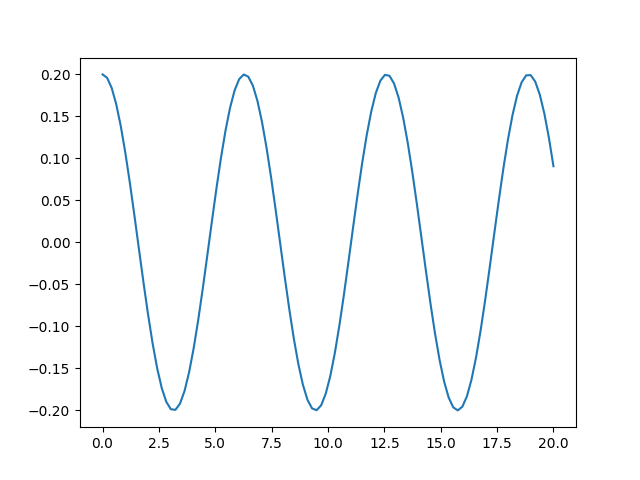
\includegraphics[scale=0.7]{mp111.png}}
\begin{changemargin}{4.5cm}{4.5cm}  
  Figure 2.1: $\implies \phi'' = -\sin{\phi}$.
\end{changemargin}
\end{center}

\begin{center}
  \makebox[0pt]{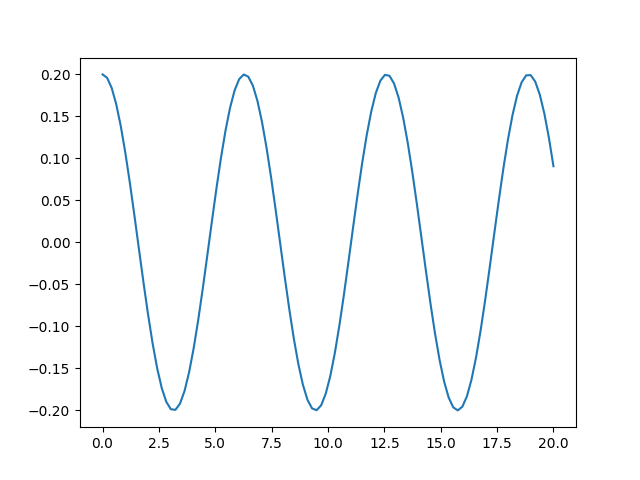
\includegraphics[scale=0.7]{mp111.png}}
\begin{changemargin}{4.5cm}{4.5cm}  
  Figure 2.1: $\implies \phi'' = -\sin{\phi} + 0.008\cos{(0.2t - \phi)}$.
\end{changemargin}
\end{center}

\newpage

\begin{center}
  \section*{4}
  \noindent\rule{16cm}{0.4pt}
  \section*{Mini-Project 2: Question 2} %\cite{Taylor2005}}
  \noindent\rule{16cm}{0.4pt}
\end{center}

\subsection*{4.1 Equations of problems}

\begin{center}
  \begin{tikzpicture}
    \draw [dotted] (1, 2) -- (1, -3);
    \draw [dotted] (-1, 2) -- (-1, -3);
    \draw [fill = white] (0, 0) rectangle (2, 1);
    \draw (0.5, -0.2) circle (0.2cm);
    \draw (1.5, -0.2) circle (0.2cm); 
    \draw [->] (-1, 2) -- (1, 2);
    \draw [<-] (1.316, -0.948) arc (-71:-90:1);
    \node at (1.19, -1.3) {$\phi$};
    \node at (1.9, -1.5) {$\vec{r_2}$};
    \draw (1, 0) -- (2, -3);
    \draw [fill=white] (2, -3) circle (0.2cm);
    \draw [decoration={aspect=0.3, segment length=3mm, amplitude=3mm,coil},decorate] (-4, 0.5) -- (-1, 0.5);
    \draw (-1, 0.5) -- (0, 0.5);
    \draw (-5, 0.5) -- (-4, 0.5);
    \draw (-5, -0.4) -- (3, -0.4); 
    \draw (-5, -0.4) -- (-5, 3); 
    \node at (-2.65, 1.2) {$k$};
    \node at (1, 0.5) {$m$};
    \node at (1.95, -3.5) {$M$};
    \node at (0, 2.3) {$\vec{r_1}$};
    \draw [->] (-7, -0.4) -- (-6, -0.4);
    \draw [->] (-7, -0.4) -- (-7, -1.4);
    \node at (-5.8, -0.4) {$x$};
    \node at (-7, -1.65) {$y$};
  \end{tikzpicture}
  \end{center}
%\textbf{$\mathcal{L}$}\textit{\textbf{agrangian}}



\subsection*{4.2 Analysis}

For the second question, we had the following Lagrangian:
\\
$\Lagr = \Lagr(\dot{x}, x, \dot{\phi}, \phi, t) = \frac{1}{2} m \dot{x}^2 + \frac{1}{2} M \dot{x}^2 + \frac{1}{2} M L^2 \dot{\phi}^2 + M \dot{x}L\dot{\phi}\cos(\phi)) - \frac{1}{2}kx^2 +MgL\cos(\phi)$

\noindent However, observe that this has five arguments, but our program works for three arguments. We could in theory generalize our program, but we will slightly modify it to work for five argument lagrangians (this limitation will be explained in the conclusion). The only limitation is not being able to convert the equation's ``raw'' form to a nicer looking equation; but, we do get an equation that we can plot.


\subsection*{4.3 Solutions - \emph{.py}}

Plugging this Lagrangian into \verb|MP2q2.py|, the program retruns the DE, we get 

\begin{lstlisting}[language = html]
  ∂ℒ/∂x        = 0


  ∂ℒ/∂x'       = 1.0*cos(phi(t))*Derivative(phi(t), t) + 1.0*x'
  
  
  d/dt(∂ℒ/∂x')  = -1.0*sin(phi(t))*Derivative(phi(t), t)**2 + 1.0*cos(phi(t))*Derivative(phi(t), (t, 2)) + 1.0*x''
  
  
  Required DE      : -1.0*sin(phi(t))*Derivative(phi(t), t)**2 + 1.0*cos(phi(t))*Derivative(phi(t), (t, 2)) + 1.0*x'' = 0
\end{lstlisting} 

\noindent \verb|-1.0*sin(phi(t))*Derivative(phi(t), t)**2 + 1.0*cos(phi(t))*Derivative(phi(t), (t, 2))|
\verb|+ 1.0*x'' = 0| \\
$\implies -\phi'^2\sin{\phi} + \phi''\cos{\phi} + x'' = 0$

We hence get the following plots: (just as in Question 2!)

\begin{center}
  \makebox[0pt]{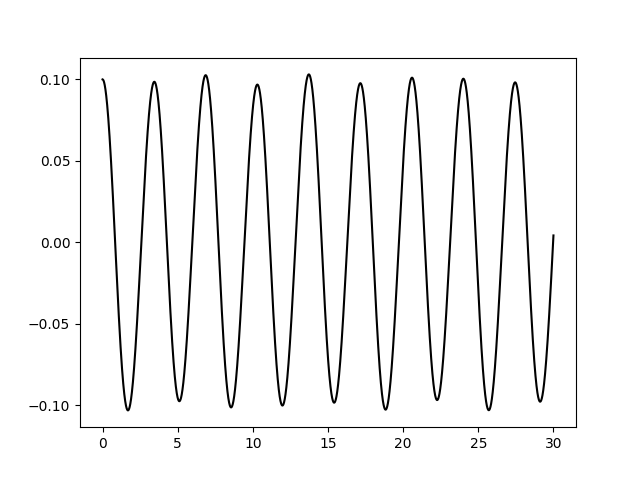
\includegraphics[scale=0.7]{mp221.png}}
\begin{changemargin}{4.5cm}{4.5cm}  
  Figure 2.1: $-\phi'^2\sin{\phi} + \phi''\cos{\phi} + x'' = 0$.
\end{changemargin}
\end{center}

\newpage

% \subsection{Taylor Example 6.2: The Brachistochrone \cite{Taylor2005}}
% This problem is both a way to showcase the workings of the method and a verification of it. Since we already know the solution to be a cycloid. 

% It requires investigation to find the path of least time between two points with one higher then the other as a particle travels between them subject to gravity. 

% The time that this particle would take to reach from A to B is:
% \begin{center}
% $t \Big\rvert_{\vec{x} = A}^{\vec{x} = B} = \displaystyle\int_{1}^{2} \cfrac{1}{v} \,ds $
% \end{center}
% Conservation of energy states that $U_{initial} = T_{final}$ which means at any point during the particle's movement the velocity can be defined by $v=\sqrt(2gy)$.
% Due to this approach v is a function with an argument of y. So it is convenient to have $y$ be the independent variable and $x$ be the function $x(y)$.

% We can now define $ds$ using vector addition of our variables.
% \begin{center}
% $ds = \sqrt{dx^2 +dy^2} = \sqrt{dx(y)^2 +dy^2} = \sqrt{x'(y)^2 +1} dy$
% \end{center}

% The time integral can now be re written as:
% \begin{center}
% $t \Big\rvert_{\Vec{x} = A}^{\Vec{x} = B} 
% \-\hspace{0.2cm}
% = \displaystyle\int_{0}^{y_2}\dfrac{\sqrt{x'(y)^2 +1}}{\sqrt{2gy}}\,dy $
% \\
% \-\hspace{1.95cm}
% $= \dfrac{1}{\sqrt{2g}} \displaystyle\int_{0}^{y_2}
% %\[ \int \]
% \dfrac{\sqrt{x'(y)^2 +1}}{\sqrt{y}} \,dy $
% \end{center}
% The Integrand represents the quantity we need to minimize so that will be out Lagrangian:
% \begin{empheq}[box={\mybluebox[5pt][5pt]}]{equation*}
%   \Lagr(x,x',y) = \sqrt{\cfrac{x'(y)^2 +1}{y}}
% \end{empheq}
% %\begin{center}
% %$\Lagr(x,x',y) = f(x,y,y') = \cfrac{\sqrt(x'(y)^2 +1)}{\sqrt(y)}$
% %\end{center}

% \subsection{Taylor Example 6.3: Shortest Path Between 2 Points Again}
% As a different approach to Taylor:6.1 we can define $x$ and $y$ as functions of $t$ where $t = time$. Due to this the Lagrangian will now be:
% \begin{empheq}[box={\mybluebox[5pt][5pt]}]{equation*}
%   \Lagr(x,x',y,y',t) = \sqrt{x'(t)^2 +y'(t)^2}
% \end{empheq}
% %\begin{center}
% %$\Lagr(x,y,y') = f(x, x', y, y', t) = \sqrt{x'(t)^2 +y'(t)^2}$
% %\end{center}


% \subsection{Mini Project 2: Question 1}
%  Consider  a  pendulum  with  mass $m$,  length $L$,  and  angle $\phi$,  attached  to  the  edge  of a  wheel  with radius $R$.  The wheel rotates with fixed angular velocity $\omega$.
%  Let the origin be the centre of the wheel and be the support point of the pendulum.

% \begin{center}
%   $\Lagr(x, x', \phi, \phi',t) = \frac{mv^2}{2} - mgy
%   \newline$ 
%     = $\cfrac{m}{2} (L^2 \phi'^2 + 2R\omega L \phi' sin(\phi-\omega t) -mg(R sin(\omega t) -L cos(\phi)) + const$
% \end{center}



% \subsection{Mini Project 2: Question 2}
% Consider a mass m attached to a spring with spring constant $k$,  and let $x$ be the displacement of the mass from its equilibrium.  A pendulum, with mass $M$, length L, and angle $\phi$, is attached to the mass $m$.

% \begin{center}
%   $\Lagr(x, x', \phi, \phi',t) = \frac{mv^2}{2} - mgy
%   \newline
%   = \frac{1}{2} (m+M)x'^2 + MLcos(\phi)x'\phi' +ML^2\phi'^2/2 - kx^2/2 + MgLcos(\phi)$
% \end{center}

\section{Conclusions}
The report shows, the program involves a 3 step process that can find how the minimization of one quantity affects a system. 
The system starts at the Lagrangian of the system defined with its independent, dependent and derivative of the dependent variable. The code will then utilize the Euler-Lagrange equations to minimize the quantity that the user defines. The relationship is then used to obtain a differential equation. For simpler problems these DEs can be solved analytically. For Problem 1 this DE states that the double derivative of the indepent variable is 0. This is correct since the solution to that DE is of the same form as the equation of a line. Which is the correct solution to the problem. 

Problem 2 does the same thing as above but instead of minimzing distance it minimizes time. And as the plot shows: the solution is the original brachistochrone that inspired this project. This verified out method and results.

Problems 3 and 4 were added to expand the complexity of the problems that the program can solve. Solutions and plots produced for those problems also match the correct solutions. 
For further development of this project, a user can potentially expand this code to include problems that involve several dependent variables parametrized by a single quantity or potentially be expanded to any arbitraty n dimensional bodies or n dimensional problems.


\begin{thebibliography}{1}

\bibitem{Taylor2005} Taylor, J. R. \textit{Classical
  Mechanics}. University Science Books, 2005. 
\bibitem{Levi2014} Mark Levi \textit{Quick! Find a Solution to the
Brachistochrone Problem}. Mathematical Curiosities, 2005. 
\bibitem{Carnier2017} Rodrigo Matos Carnier \textit{Energy-efficient optimal control of robotic gait by indirect methods}. Research Gate , 2017

\end{thebibliography}


\end{document}
